\documentclass[oneside,a4paper,english,links]{amca}
%
\usepackage{graphicx}
\usepackage{amsmath,amsfonts}
\usepackage[utf8]{inputenc}
%
\title{INSTRUCTIONS TO PREPARE AN ARTICLE ACCORDING TO THE AMCA-STYLE}


\author[a]{L.C. Agorio}
\author[b]{M.C. Vanzulli}
\author[c]{B. Bazzano}
\author[c]{Jorge M. Pérez Zerpa}
%
\affil[a]{Instituto de Ingeniería Eléctrica, Facultad de Ingeniería, Universidad de la República, Montevideo, Uruguay}

\affil[b]{Instituto de Ingeniería Mecánica y Producción Industrial, Facultad de Ingeniería, Universidad de la República, Montevideo, Uruguay}
%
\affil[c]{Instituto de Estructuras y Transporte, Facultad de Ingeniería, Universidad de la República, Montevideo, Uruguay}

\begin{document}
\vspace{3cm}

\maketitle

\begin{keywords}
Artificial Neural Networks, Finite Element Method, Solid Mechanics, Surrogate-models.
\end{keywords}

\begin{abstract}
    Solving finite element simulations can be computationally expensive, particularly in solid mechanics field. This is a challenge in applications such as bio-mechanics and manufacturing design process, where the same problem may need to be solved in real time for different configurations or input data.  In this paper we combined Finite Element Method (FEM) and Artificial Neural Networks (ANN) to improve the speed and efficiency of solving mechanical problems. A pipeline to generate databases of FEM solutions was developed interacting with an in-house Open Source Software for non-linear Analysis of Structures (ONSAS). The databases were used to train a neural network that takes geometrical and material properties as inputs, and as an output predicts the displacements solution of the mechanical problem. Our experiments showed that the proposed approach was effective, achieving low losses on both the training and test datasets. We present a validation example where the ANN was capable to match the analytic solution with great accuracy. Moreover, more complex problems were solved with different geometries, boundary conditions and materials considering large strain deformations. One advantage of our implementation is its simplicity and scalability. We were able to develop a pipeline that can be easily scaled to a wide range of mechanical problems. Additionally, the use of ANN allows a faster computation times than the traditional solvers using the FEM method.  Although the study presents promising results, we also discussed the limitations of the proposed approach and potential directions for future work.
\end{abstract}

%\section{INTRODUCTION}
%
%This document provides information and instructions to prepare an
%article according to the AMCA style. Only the articles formatted
%according to the present guidelines will be accepted for AMCA
%publications.
%
%\section{GENERAL SPECIFICATIONS}
%
%The article may be written in English, Spanish or Portuguese
%within a printing box of 16cm x 24cm, centered in the page. The
%paper including figures, tables and references must have a minimum
%length of 4 pages and must not exceed 10 pages. The article must
%be uploaded to the AMCA site in the form of a \textbf{PDF} file;
%no other formats (MS Word, RTF) are accepted. The size of the PDF
%file of the article must not exceed 2~MBytes.
%
%\subsection{Use of acronyms}
%
%If acronyms are used, then define them before their first
%occurrence.
%
%\section{TITLE, AUTHORS, AFFILIATION, KEYWORDS}
%
%The first page must contain the Title, Author(s), Affiliation(s),
%Keywords and the Abstract. The second page must begin with the
%Introduction. The first line of the title is located 3cm from the
%top of the printing box to enable the insertion of the conference
%header and AMCA logo.
%
%\subsection{Title}
%
%The title should be written centered, in 14pt, boldface Times
%Roman, all capital letters. It should be single spaced if the
%title is more than one line long. Inclusion of formulas or special
%characters in the title is \textbf{highly} discouraged. Acronyms
%may be used if defined \emph{in-line}, for instance ``Large Eddy
%Simulation (LES) of flow around a cylinder''.
%
%\subsection{Author}
%
%The author's name should include first name, only the initial of
%the second name and last name. It should be written centered, in
%12pt boldface Times Roman, 12pt below the title. Collate all the
%authors together, split in several lines if necessary. Use the
%connector ``{\bf and}'' before the last author. Affiliations must
%be arranged in centered blocks, after the list of authors.
%Identify the authors with their corresponding affiliations using a
%letter superscript, as in the example. If all the authors belong
%to the same affiliation do not use superscript
%
%\subsection{Affiliation}
%
%Author's affiliation should be written centered, in 11pt Italic
%Times Roman, 12pt below the list of authors. A 12pt space should
%separate two different affiliations. It is recommended that the
%authors include an e-mail address and a web page per affiliation
%site, if possible.
%
%\subsection{Keywords}
%
%Please, write no more than six keywords.  They should be written
%left aligned, in 12pt Times Roman, and the line must begin with
%the word {\bf Keywords}. A 12pt space should separate the keywords
%from the affiliations.
%
%\subsection{Abstract}
%
%Use 11pt Times Roman for the abstract. The word {\bf Abstract}
%must be set in boldface, not italicized, at the beginning of the
%first line. The abstract text should be justified and separated
%12pt from the keywords, as shown in the first page of these
%instructions. The abstract should be self-contained, so do not
%include figures, tables or equations in the abstract. Neither
%include any reference to such material. It is discouraged to
%include references to other work in the abstract. In case of
%including any references, then they should be included
%\emph{in-line} but abbreviated, as in this example (C. Jhonson
%et.al., \emph{Int J Num Meth Eng}, 34(3):543--568 (1992); D.
%Mitchell and J. Brady, \emph{J Sound Vib}, 21(2):221--230 (2006)).
%Multiple citations should be separated by semi-colons. \textbf{It
%is strongly discouraged to include more than 2 references in the
%abstract}. Inclusion of formulas is \textbf{highly} discouraged.
%Avoid special characters. If acronyms are used, then define them
%before their first occurrence. An extension of the abstract
%between 150 and 300 words is suggested.
%
%\section{HEADINGS}
%
%\subsection{Main headings}
%
%The main headings should be written left-aligned, in 12pt,
%boldface and all capital Times Roman letters. There should be a
%12pt space before and a 6pt space after the main headings.
%
%\subsection{Secondary headings}
%
%The secondary headings should be written left-aligned, in 12pt,
%boldface Times Roman, with an initial capital for the first word
%only. There should be a 12pt space before and a 6pt space after
%the secondary headings.
%
%\section{TEXT}
%
%The normal text should be written single-spaced, justified, using
%12pt Times Roman, in one column. The first line of each paragraph
%must be indented 0.5cm. There is not inter-paragraph spacing.
%
%\section{PAGE NUMBERS}
%
%The authors {\bf must not number} the pages of the article.
%Numbers will be added by the editor/publisher.
%
%\section{FIGURES}
%
%All the figures should be numbered consecutively and captioned.
%The caption should be written centered, in 10pt Times Roman.
%Capitalize only the first letter of the sentence.
%
%\begin{figure*}[htb]
%\centerline{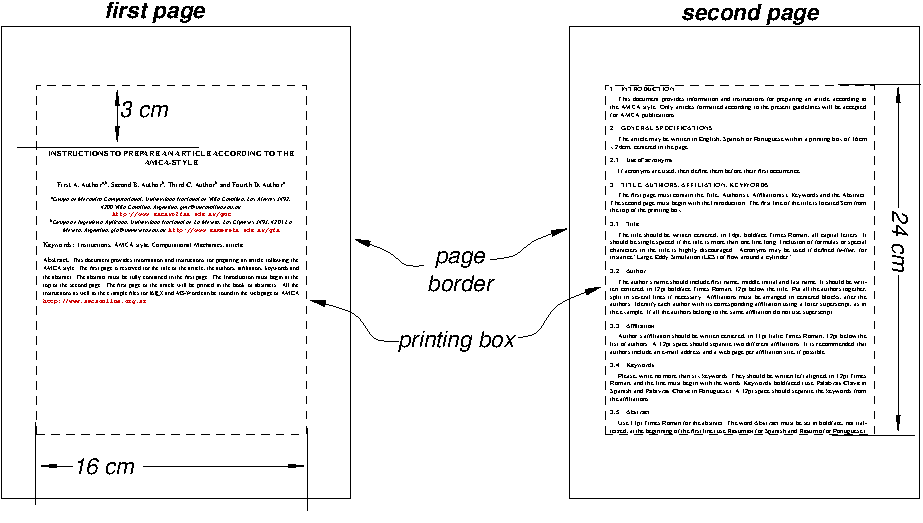
\includegraphics{firstpage}}
%\caption{Page layout}
%\label{fg:figure}
%\end{figure*}
%
%A 6pt space should separate the figure from the caption, and a
%12pt space should separate the upper part of the figure and the
%bottom of the caption from the surrounding text (see
%Fig.~\ref{fg:figure}).
%
%Figures should be referenced in the text. Color figures are
%welcomed.
%
%\section{EQUATIONS}
%
%A displayed equation is numbered, using Arabic numbers in
%parentheses. It should be  centered, leaving a 6pt space above and
%below to separate it from the surrounding text.
%
%The following example is a simple single line
%equation
%%
%\begin{equation}
%Ax = b.
%\end{equation}
%
%The next example is a multi-line equation
%%
%\begin{equation} \label{eq:simple}
%\begin{aligned}
%Ax& = b,\\
%Ax& = c.
%\end{aligned}
%\end{equation}
%%
%If possible, internal PDF links must be generated for references to
%equations. The recommended color for links to references in the text
%is blue (e.g., see Eq.~(\ref{eq:simple})).
%
%\section{TABLES}
%
%All tables should be numbered consecutively and captioned; the
%caption should be 10pt Times Roman. Capitalize only the first
%letter of the sentence.
%
%A space of 6pt separates the table from the caption, and 12pt space
%separates the table from the surrounding text. For an example, see
%Table~\ref{tab:n50}. Tables should be referenced in the text.
%
%\begin{table}[htb]
%\centering
%\begin{tabular}{|c|c|c|c|}
%\hline  & 20x20 mesh & 50x50 mesh & 100x100 mesh\\
%\hline
%\hline
% 0 & 41.00 & 1.00 & 4.92\\
%\hline
% 1 & 40.86 & 1.02 & 4.88 \\
%\hline
%10 & 23.81 & 3.44 & 2.92 \\
%\hline
%50 & 5.62 & 64.20 & 1.08 \\
%\hline
%\end{tabular}
%\caption{Condition number for the Stekhlov operator. }
%\label{tab:n50}
%\end{table}
%
%\section{FORMAT OF REFERENCES}
%
%References should be quoted in the text using the
%\emph{author-style} (a.k.a. \emph{Harvard style}). References can
%be cited in \emph{parenthetical} form
%\citep{zienkiewicz91,idelsohn94,meyer82,meyer82b}, or in
%\emph{textual} form, e.g. see
%\citet{zienkiewicz91,idelsohn94,meyer82,meyer82b}.  References are
%grouped together and sorted alphabetically at the end of the
%article as shown in these instructions. Do not include references
%that are not cited in the article body. Use references with Roman
%symbols. Do not use, for example, Greek, Chinese or Japanese
%symbols.
%
%If possible, internal PDF links must be generated for citations. The
%recommended color for links to references in the text is blue. The
%preferred color for links to external references, as web pages,
%is red (e.g. \url{http://www.amcaonline.org.ar}).
%
%\section{CONCLUSIONS}
%
%Template files in TeX, \LaTeX{} and MS-Word may be found at the
%AMCA web site: \url{http://www.amcaonline.org.ar}. It is
%recommended to use these files to comply with the style more
%easily. Remember: {\bf Do not number the pages.}
%
%%\section*{ACKNOWLEDGEMENTS} The authors acknowledges to ...
%% ACKNOWLEDGEMENTS FOR FULL ARTICLES

\bibliography{amcapaper}
\end{document}
